\section{Experimental Results and Discussion}
\label{results}

\subsection{Camera Calibration Performance}
To establish the baseline internal camera model, a robust 10-frame image dataset was processed for geometric calibration. Frames exhibiting severe optical distortion or fewer than 49 detectable corners were discarded during outlier screening. The calibration pipeline achieved a mean reprojection error of 0.1152~pixels ($\sigma = 0.0076$~pixels), confirming high geometric modeling accuracy. A representative calibration visualization following feature extraction and homography alignment is illustrated in \figref{fig:Calib}.

\begin{figure}[ht]
	\centering
	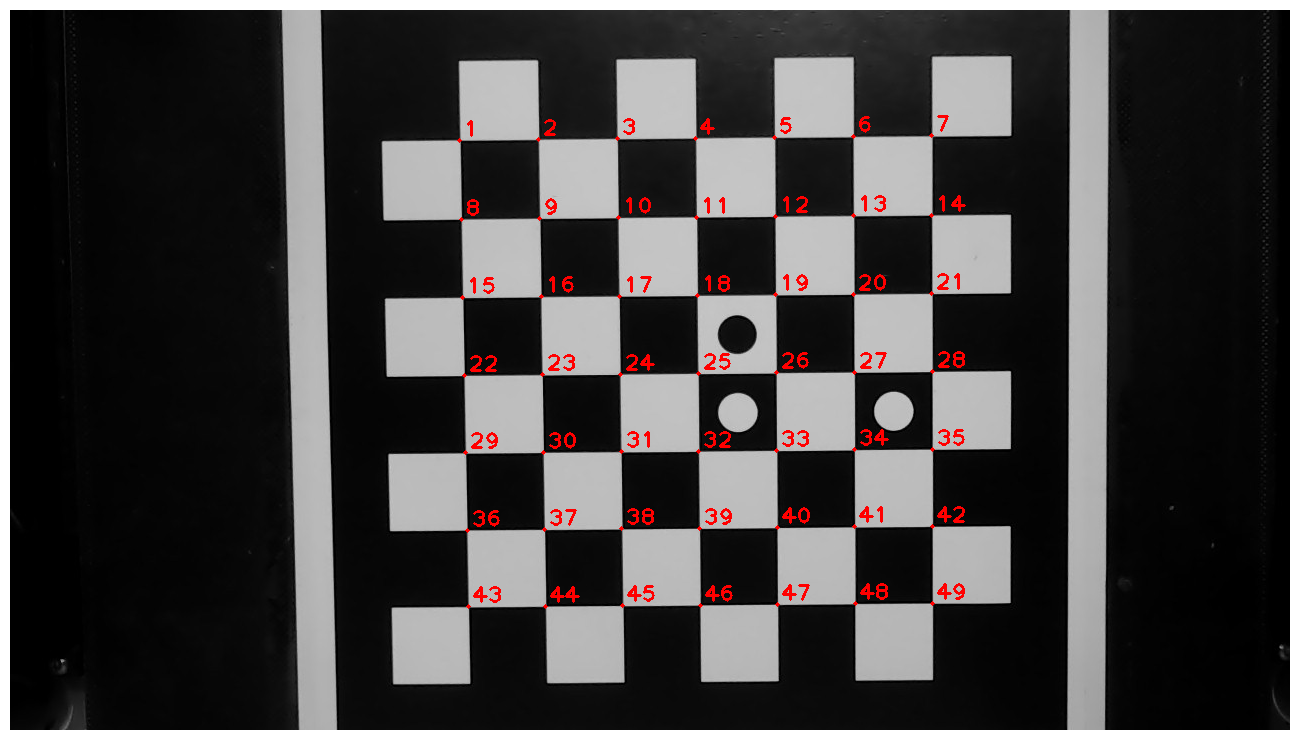
\includegraphics[width=0.8\linewidth]{images/result_after_corner_sorting.png}
	\caption{Calibration visualization following feature extraction and homography alignment.}
	\label{fig:Calib}
\end{figure}

The estimated internal camera parameters, comprising the intrinsic camera matrix $K$ and the lens distortion vector $D$, were resolved as \eqref{eq:intrinsic_matrix} and \eqref{eq:distortion_coeffs}:

\begin{equation}
	\label{eq:intrinsic_matrix}
	K = \begin{bmatrix} 2314.64 & 0 & 637.08 \\ 0 & 2328.29 & 222.87 \\ 0 & 0 & 1 \end{bmatrix}
\end{equation}

\begin{equation}
	\label{eq:distortion_coeffs}
	D = \begin{bmatrix} -0.0561 & 0.9595 & 0.0001 & 0.0004 \end{bmatrix}
\end{equation}

As derived in \eqref{eq:intrinsic_matrix}, the close match between the directional focal lengths ($f_x = 2314.64$ and $f_y = 2328.29$) confirms a uniform 1:1 sensor aspect ratio. Furthermore, the coefficients in \eqref{eq:distortion_coeffs} reveal a distinct mustache distortion profile resulting from the alternating signs between the radial distortion parameters $k_1$ and $k_2$.

\subsection{Measurement Error and Noise Floor Analysis}
The experimental displacement tracking performance was evaluated against physical dial gauge measurements over a 0.5~mm travel range. The visual output display from the position extraction pipeline of the virtual encoder is illustrated in \figref{fig:positionextraction}. The statistical measurement comparison across all evaluation cycles is presented in \figref{fig:position_comparison}. Empirical validation confirms an absolute measurement error of $3.55~\mu\text{m}$ for the X-axis and $6.25~\mu\text{m}$ for the Y-axis.

\begin{figure}[ht]
	\centering
	\subfloat[]{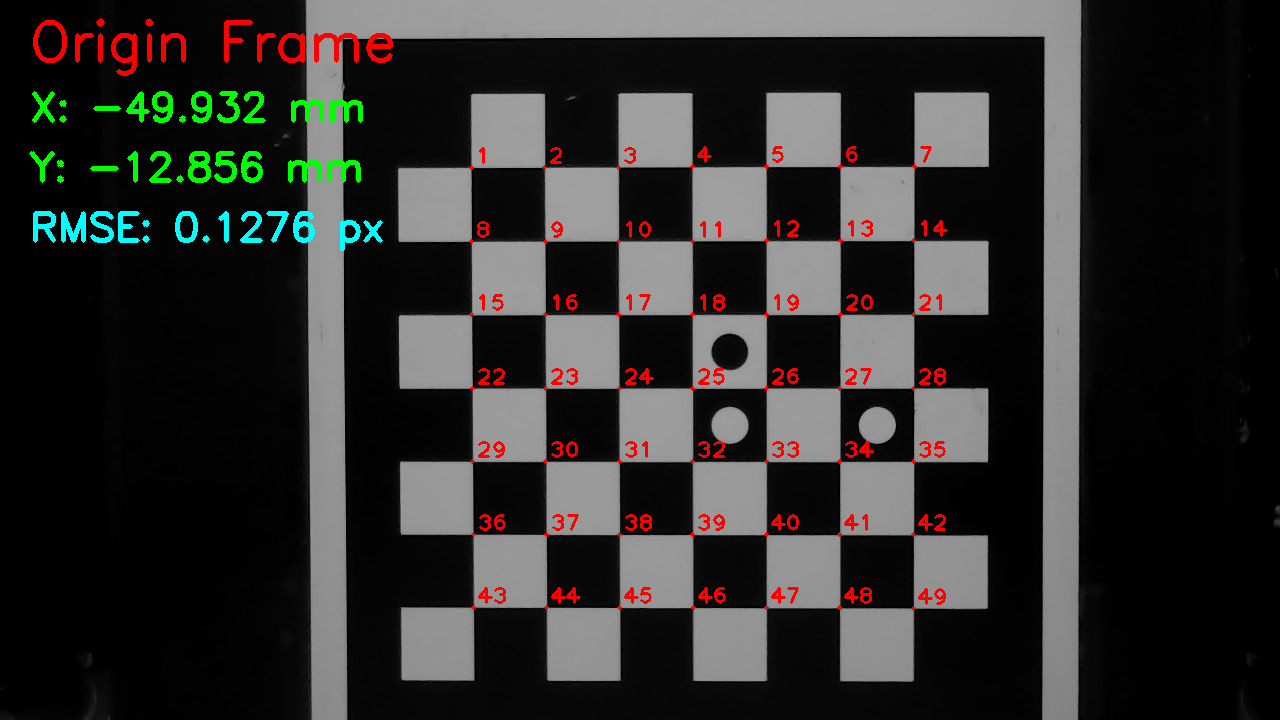
\includegraphics[width=0.75\linewidth]{images/visualisasi_ori.png}\label{fig:vis_ori}}
	\\
	\subfloat[]{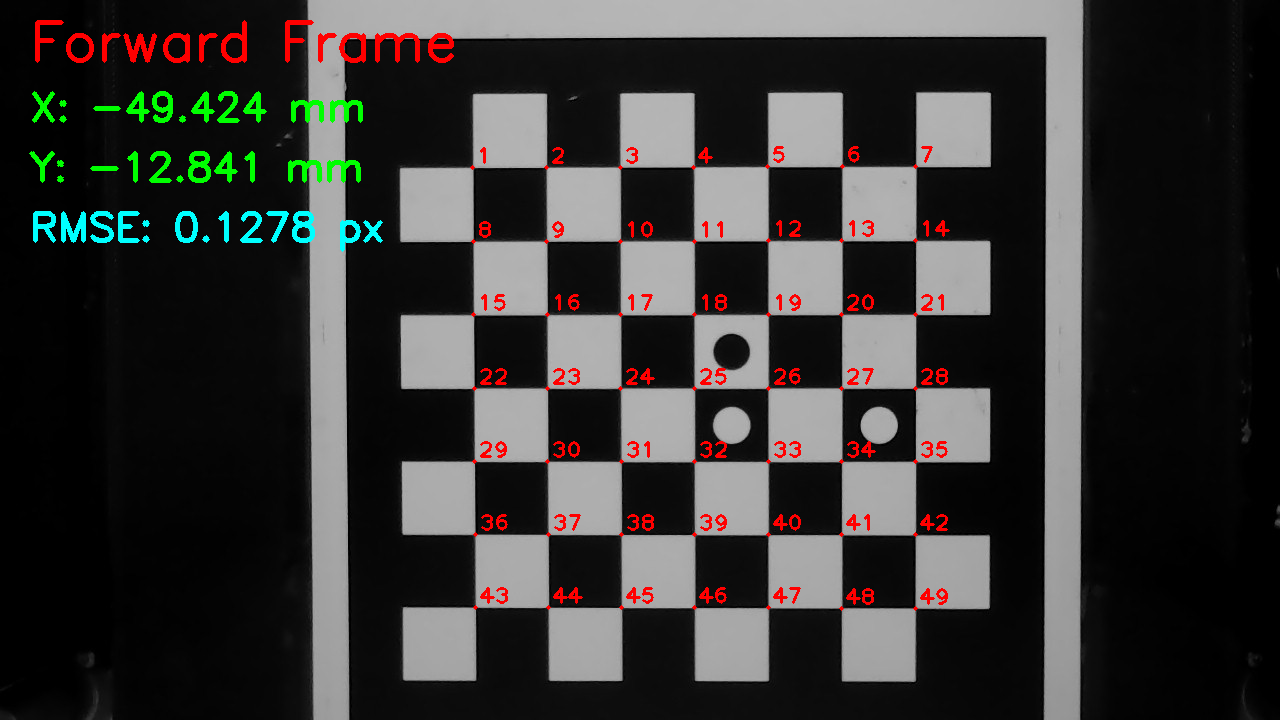
\includegraphics[width=0.75\linewidth]{images/visualisasi_fwd.png}\label{fig:vis_fwd}}
	\\
	\subfloat[]{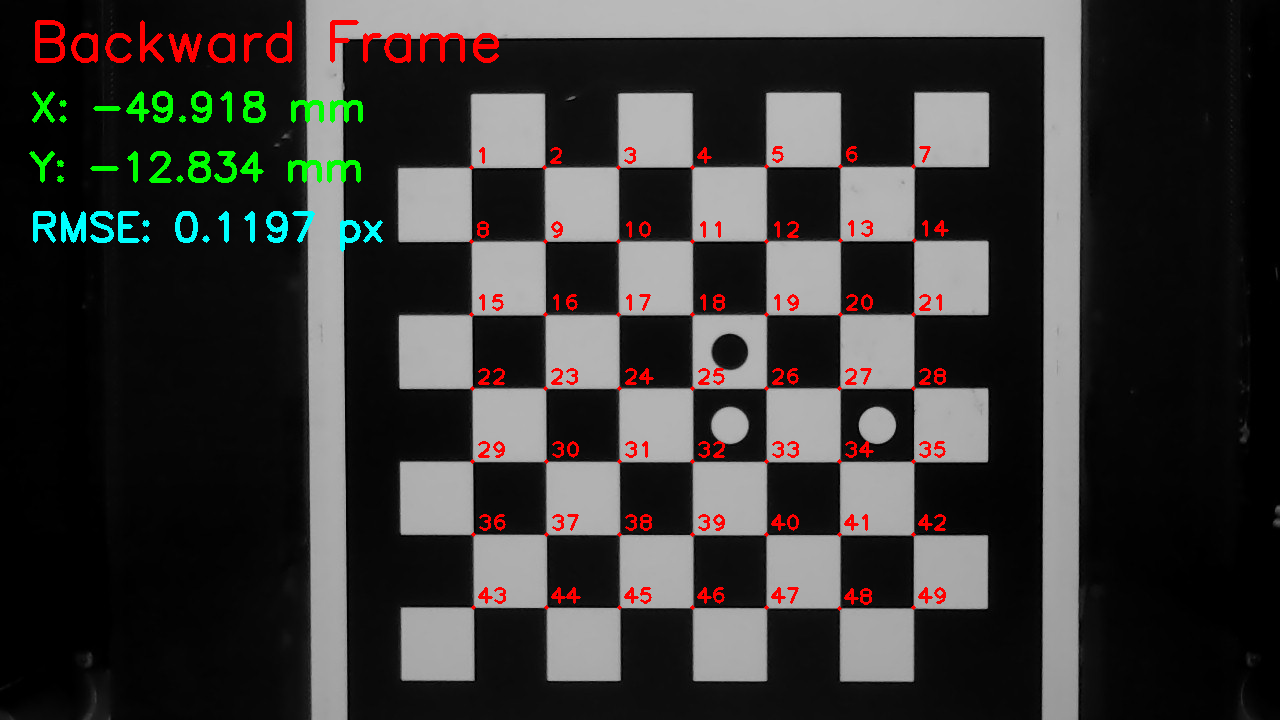
\includegraphics[width=0.75\linewidth]{images/visualisasi_bck.png}\label{fig:vis_bck}}
	\caption{Visualization of position extraction from virtual encoder process on one of the axes: (a) original frame position, (b) forward frame position, and (c) backward frame position.}
	\label{fig:positionextraction}
\end{figure}

\begin{figure}[t]
	\centering
	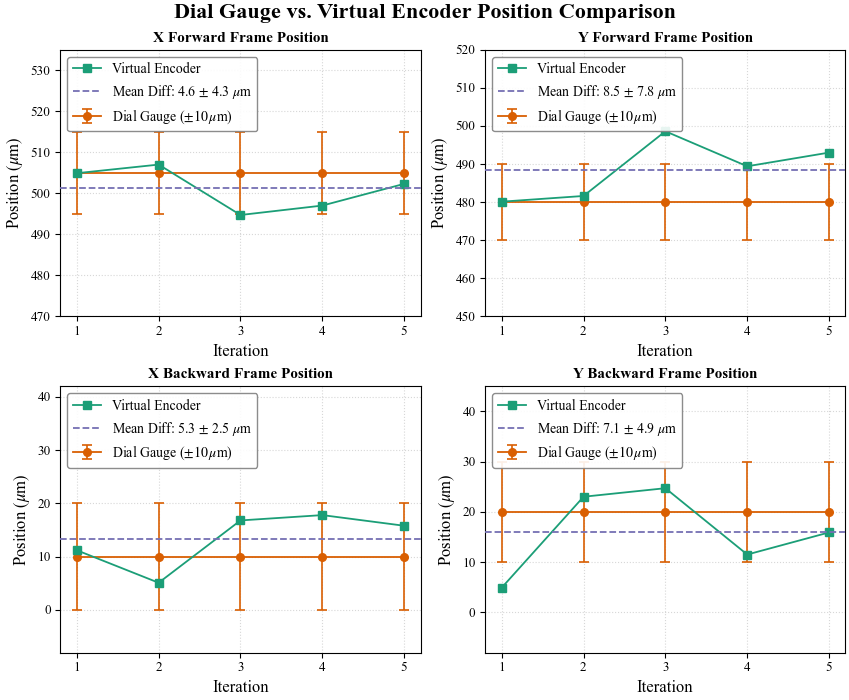
\includegraphics[width=1\linewidth]{images/1_4_position_comparison_combined.png}
	\caption{Comparison of position measurements between the dial gauge and virtual encoder across X and Y axes: forward frame position, Y forward frame position, X backward frame position, and Y backward frame position.}
	\label{fig:position_comparison}
\end{figure}

Static environmental testing under stationary conditions (\figref{fig:Noise}) yielded an internal static noise floor of $2.58~\mu\text{m}$ ($\sigma = 2.50~\mu\text{m}$) for the X-axis and $4.97~\mu\text{m}$ ($\sigma = 3.30~\mu\text{m}$) for the Y-axis. This physical deviation stems primarily from localized ambient illumination variations and structural micro-vibrations in the machine chassis. 

Based on the OV9821 sensor hardware specification with a physical pixel pitch $p_{\text{sensor}} = 3.0~\mu\text{m}$, the intrinsic focal length $f_x = 2314.64~\text{pixels}$ converts to an effective focal length $f \approx 6.94~\text{mm}$. At a fixed camera working distance $Z = 260~\text{mm}$, the physical projection scale on the print bed plane translates to $112.33~\mu\text{m/pixel}$. Consequently, the measured static noise floor corresponds to an equivalent sub-pixel detection sensitivity of $0.023~\text{pixels}$ (X-axis) and $0.044~\text{pixels}$ (Y-axis). On the physical CMOS sensor plane, a target displacement error of $2.58~\mu\text{m}$ projects to a sub-diffraction physical shift of merely $68.8~\text{nm}$ ($2.58~\mu\text{m} \times M$, where optical magnification $M = 0.0267$), demonstrating the sub-pixel precision of the EDLines corner detection pipeline. Across the $0.5~\text{mm}$ operational displacement range, the virtual encoder achieves a spatial signal-to-noise ratio ($\text{SNR}_{\text{spatial}}$) of $45.75~\text{dB}$ for the X-axis and $40.05~\text{dB}$ for the Y-axis.

\begin{figure}[tbp]
	\centering
	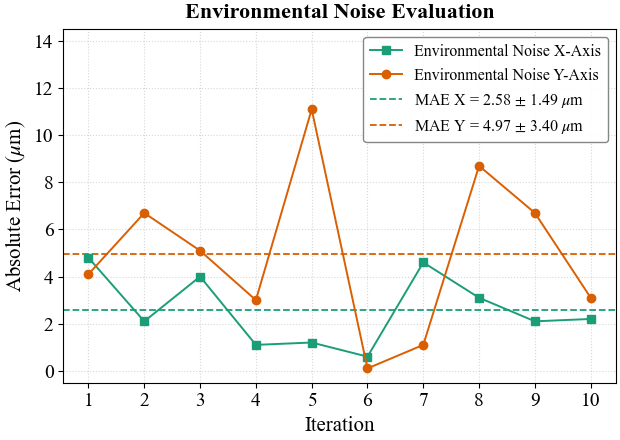
\includegraphics[width=0.8\linewidth]{images/Noise_Lingkungan.png}
	\caption{System noise floor characterization measured under stationary static testing for X and Y axes.}
	\label{fig:Noise}
\end{figure}

To comprehensively evaluate the metrological performance of the proposed virtual encoder system, both Type A and Type B measurement uncertainties were systematically quantified. The evaluation incorporates individual contributions arising from experimental repeatability, static optical noise, sub-pixel reprojection residuals, and reference hardware tolerances. The populated measurement uncertainty budget, structured according to the GUM formulation in \eqref{eq:gum_uc} and \eqref{eq:gum_expanded}, is summarized in \tabref{tab:uncertainty_budget}.

\begin{table}[tbp]
	\centering
	\caption{Measurement Uncertainty Budget for the Virtual Encoder System (ISO/IEC Guide 98-3 GUM)}
	\label{tab:uncertainty_budget}
	\scriptsize
	\setlength{\tabcolsep}{2.5pt}
	\renewcommand{\arraystretch}{1.2}
	
	\begin{tabularx}{\linewidth}{@{} L c c c c @{}}
		\toprule
		\textbf{Source of Uncertainty} & \textbf{Symbol} & \textbf{Distribution} & \textbf{X ($\mu$m)} & \textbf{Y ($\mu$m)} \\ 
		\midrule
		Measurement Repeatability (Type A) & $u_A$ & Normal ($N=5$) & 1.52 & 2.66 \\
		Static Optical Noise Floor & $u_{\text{noise}}$ & Normal & 1.49 & 3.40 \\
		Sub-pixel Reprojection Residual & $u_{\text{reproj}}$ & Normal & 2.96 & 2.96 \\
		Reference Dial Gauge Tolerance & $u_{\text{dial}}$ & Rectangular ($\sqrt{3}$) & 5.77 & 5.77 \\ 
		\midrule
		\textbf{Combined Std. Uncertainty ($u_c$)} & $u_c$ & Normal & \textbf{6.83} & \textbf{7.61} \\
		\textbf{Expanded Uncertainty ($U, k=2$)} & $U$ & Normal ($95\%$) & \textbf{13.66} & \textbf{15.22} \\ 
		\bottomrule
	\end{tabularx}
\end{table}

As indicated in \tabref{tab:uncertainty_budget}, the calculated expanded measurement uncertainty at a 95\% confidence level ($k=2$) is $13.66~\mu\text{m}$ along the X-axis and $15.22~\mu\text{m}$ along the Y-axis. Quantitative analysis of the budget components reveals that the physical reference instrument (dial gauge resolution tolerance) constitutes the primary Type B uncertainty contribution ($5.77~\mu\text{m}$). Conversely, the intrinsic optical uncertainty of the virtual encoder is maintained below $3.0~\mu\text{m}$, benefiting from the spatial corner-averaging effect inherent to the $7 \times 7$ chessboard marker array. Consequently, these findings confirm that the primary bottleneck in system accuracy arises from mechanical calibration limits rather than the vision-based tracking pipeline.

\subsection{Baseline Evaluation and Fine-Tuning Outcomes}
Initial testing of the uncalibrated machine revealed significant motion discrepancies. The default X-axis profile exhibited a forward travel error of $46.3~\mu$m and a backlash error of $12.4~\mu$m. The Y-axis displayed larger deviations, with a forward travel error of $55.0~\mu$m and a backlash gap of $24.4~\mu$m. Notably, structural axis skew introduced massive parasitic drifts under single-axis travel, showing an X-on-Y drift angle of $-0.5344^\circ$ and a Y-on-X drift angle of $0.5171^\circ$.

\begin{table}[b]
	\centering
	\caption[Fine-Tuned Calibration Parameters]{Fine-Tuned Calibration Parameters}
	\label{tab:parameter_final_kalibrasi}
	\footnotesize
	
	\begin{tabularx}{\linewidth}{@{} l X c @{}}
		\toprule
		\textbf{Parameter} & \textbf{Description} & \textbf{Final Value} \\
		\midrule
		\texttt{STEPX}        & X-axis step resolution & 79.72 \textit{steps/mm} \\
		\texttt{STEPY}        & Y-axis step resolution & 80.40 \textit{steps/mm} \\
		\midrule
		\texttt{BACKLASH\_X} & X-axis backlash compensation & 13.3 $\mu$m \\
		\texttt{BACKLASH\_Y} & Y-axis backlash compensation & 31.4 $\mu$m \\
		\midrule
		\texttt{SKEW\_X\_ON\_Y} & Parasitic X-drift during Y motion & -9.2 $\mu$m/mm \\
		\texttt{SKEW\_Y\_ON\_X} & Parasitic Y-drift during X motion & 9.213 $\mu$m/mm \\
		\bottomrule
	\end{tabularx}
\end{table}

\begin{figure}[t]
	\centering
	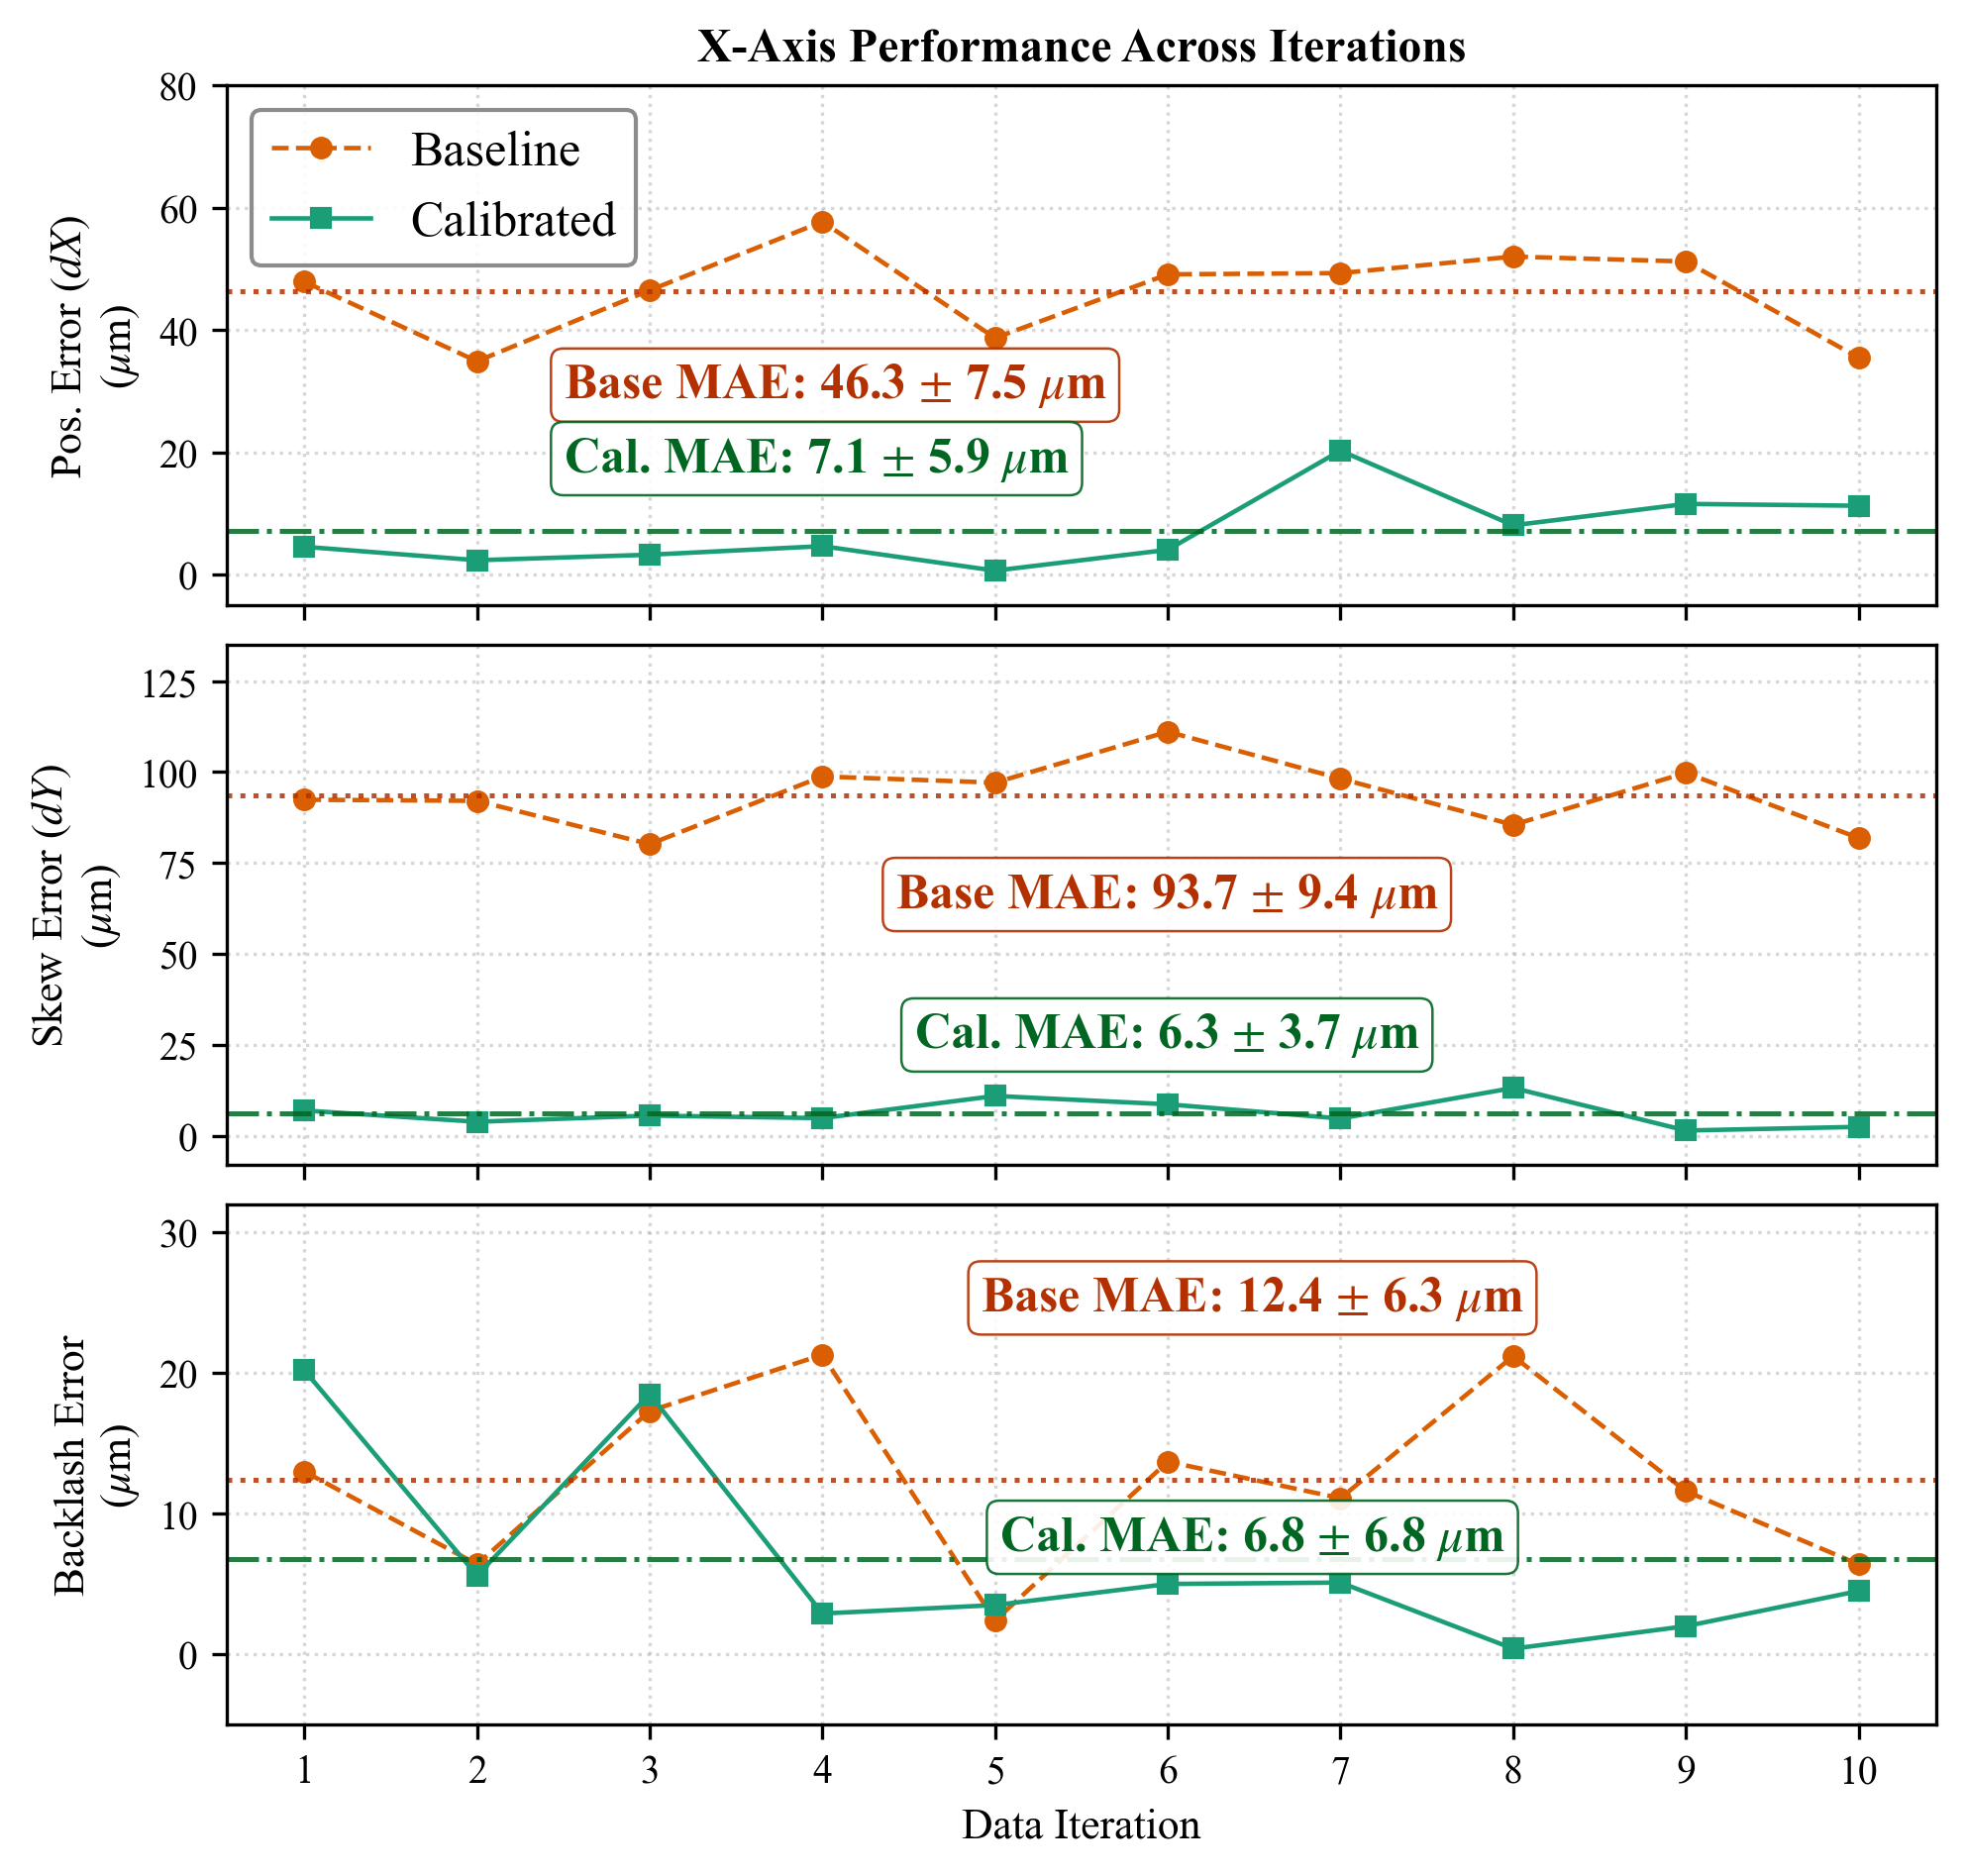
\includegraphics[width=1\linewidth]{images/x_axis_iterations.png}
	\caption{X-axis single-axis error tracking across 10 iterations comparing baseline and calibrated states for positioning, skew, and backlash parameters.}
	\label{fig:x_axis_iter}
\end{figure}

\begin{figure}[t]
	\centering
	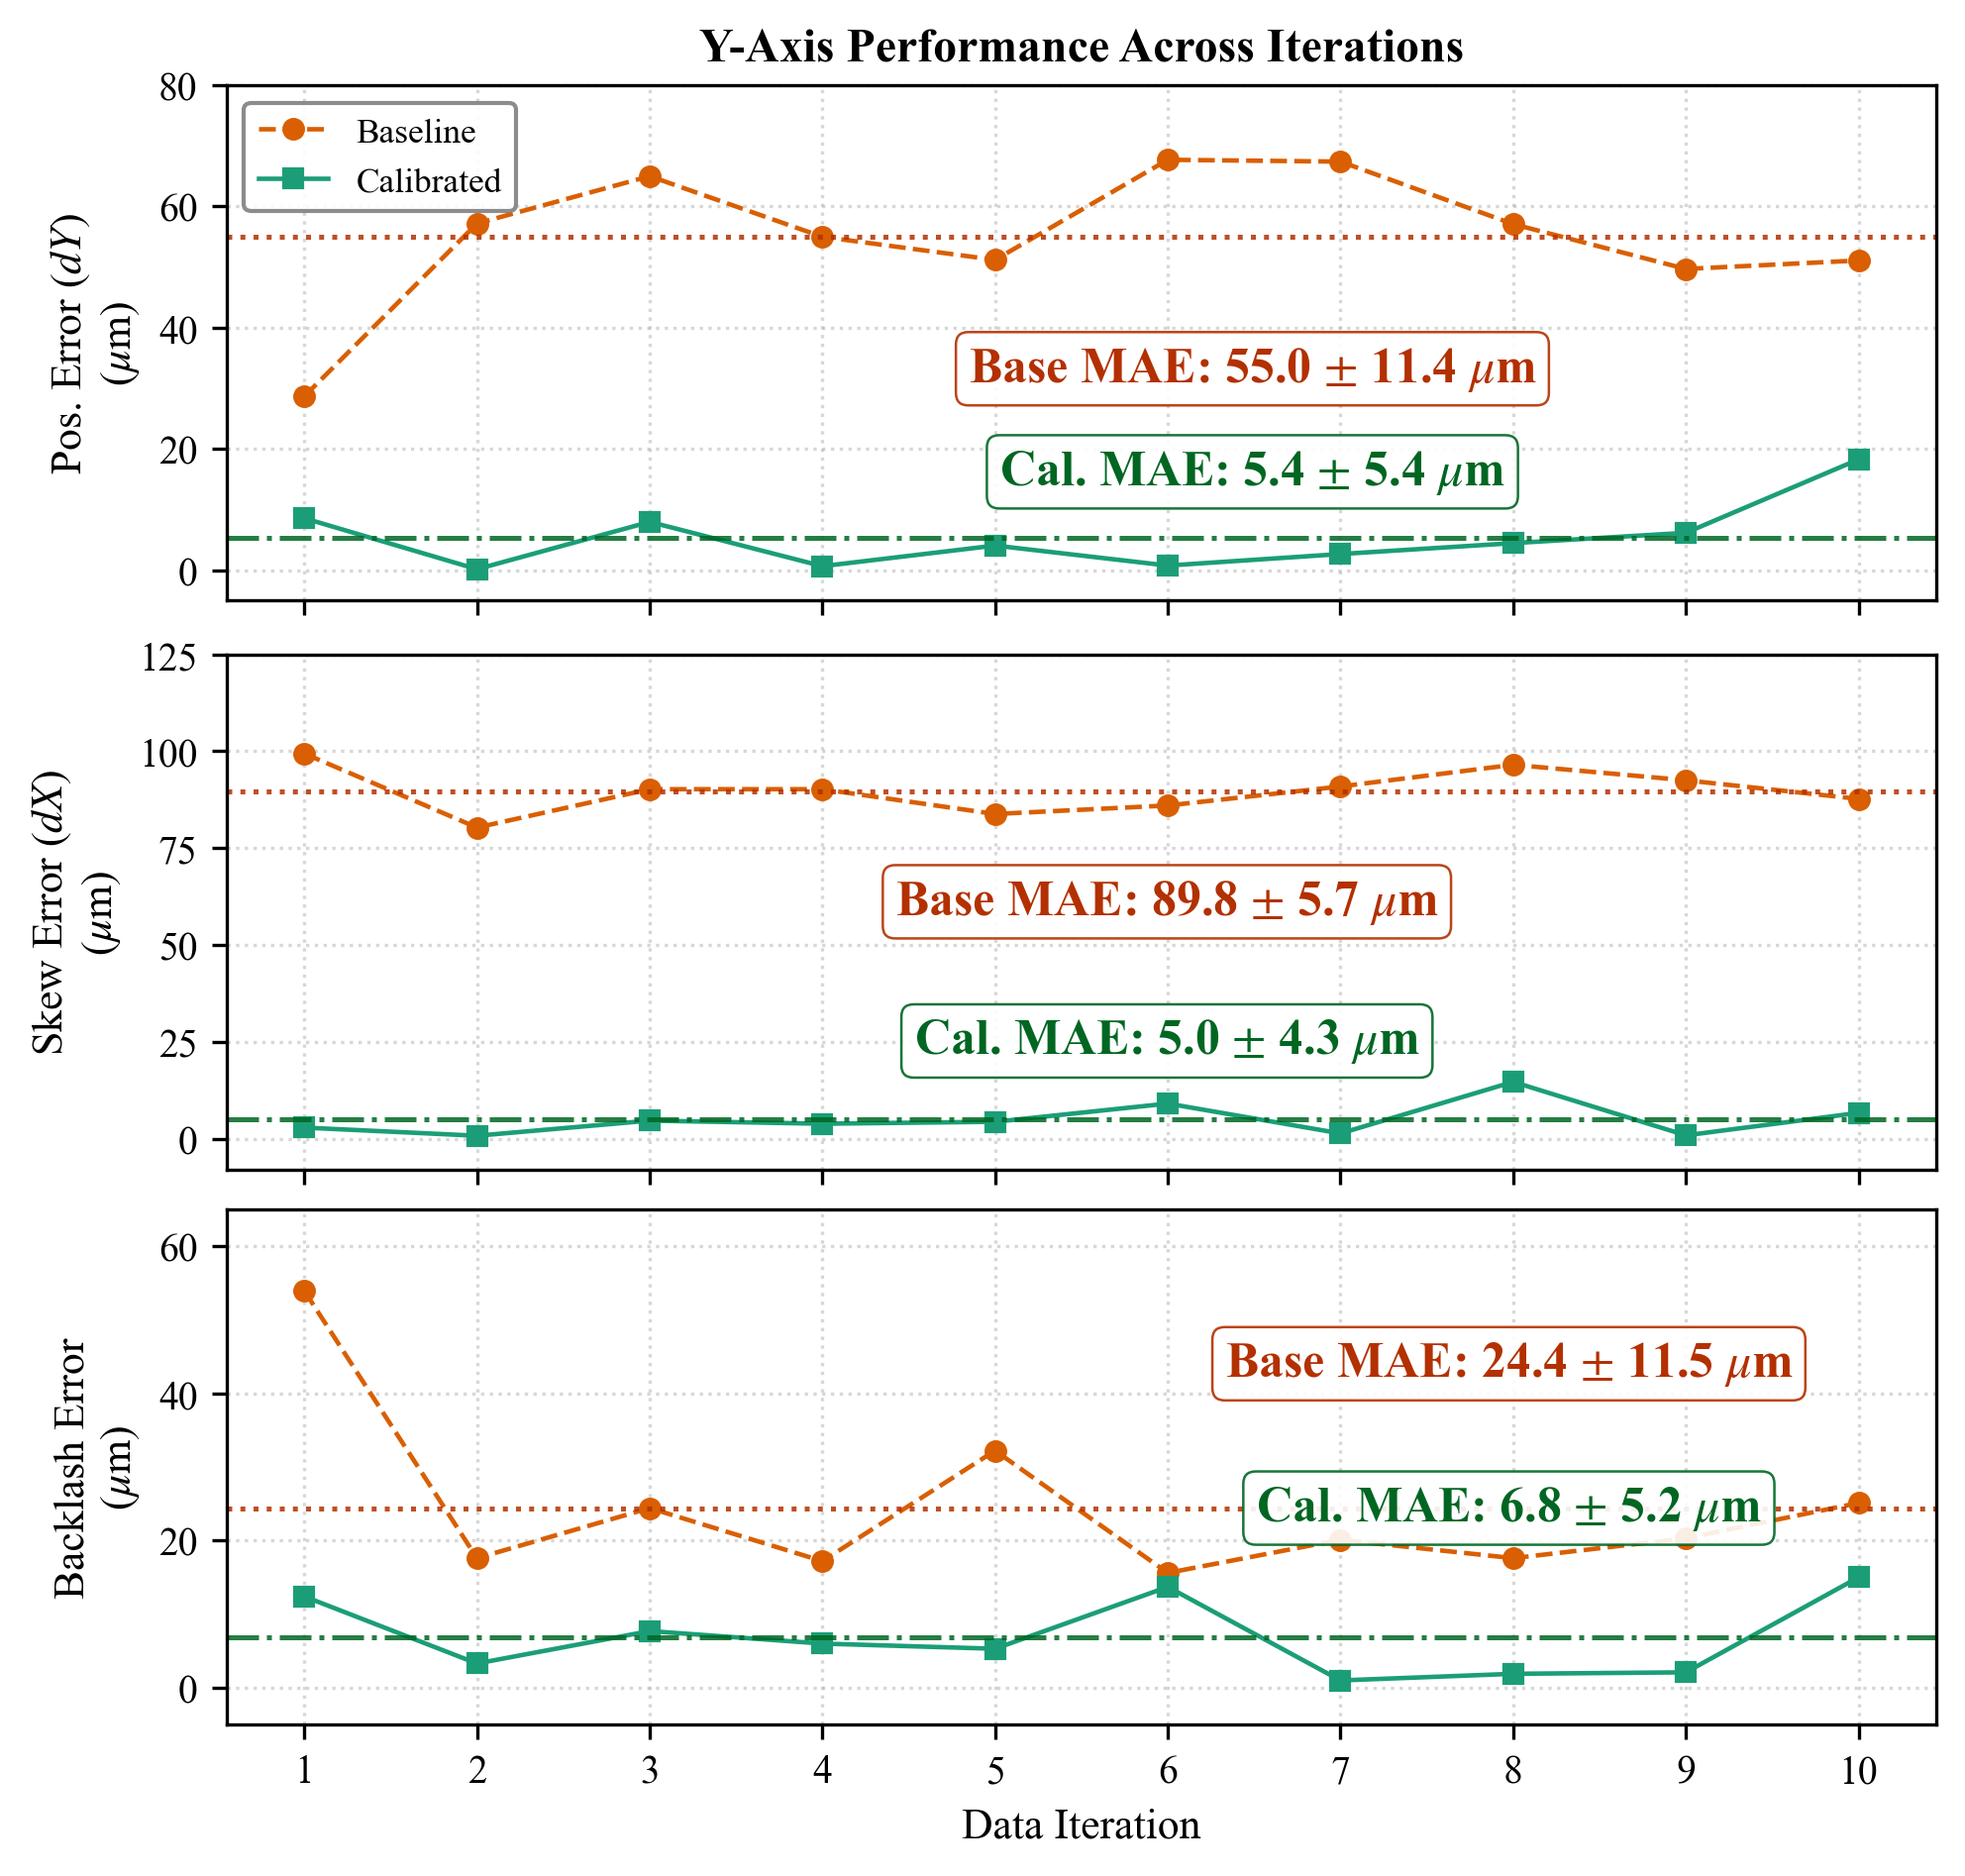
\includegraphics[width=1\linewidth]{images/y_axis_iterations.png}
	\caption{Y-axis single-axis error tracking across 10 iterations comparing baseline and calibrated states for positioning, skew, and backlash parameters.}
	\label{fig:y_axis_iter}
\end{figure}

Iterative fine-tuning systematically optimized the calibration constants over multiple correction cycles until a steady-state condition was reached. The final operational parameters converged at $79.72~\text{steps/mm}$ for the X-axis and $80.40~\text{steps/mm}$ for the Y-axis, with backlash compensations set to $13.3~\mu$m and $31.4~\mu$m, respectively. Cross-talk skew factors stabilized symmetrically at $\pm 9.2~\mu$m/mm. As shown in \figref{fig:maesum}, this optimization reduced linear axis errors to single-digit micrometers, matching the limits of the system's measurement resolution.

\begin{figure}[t]
	\centering
	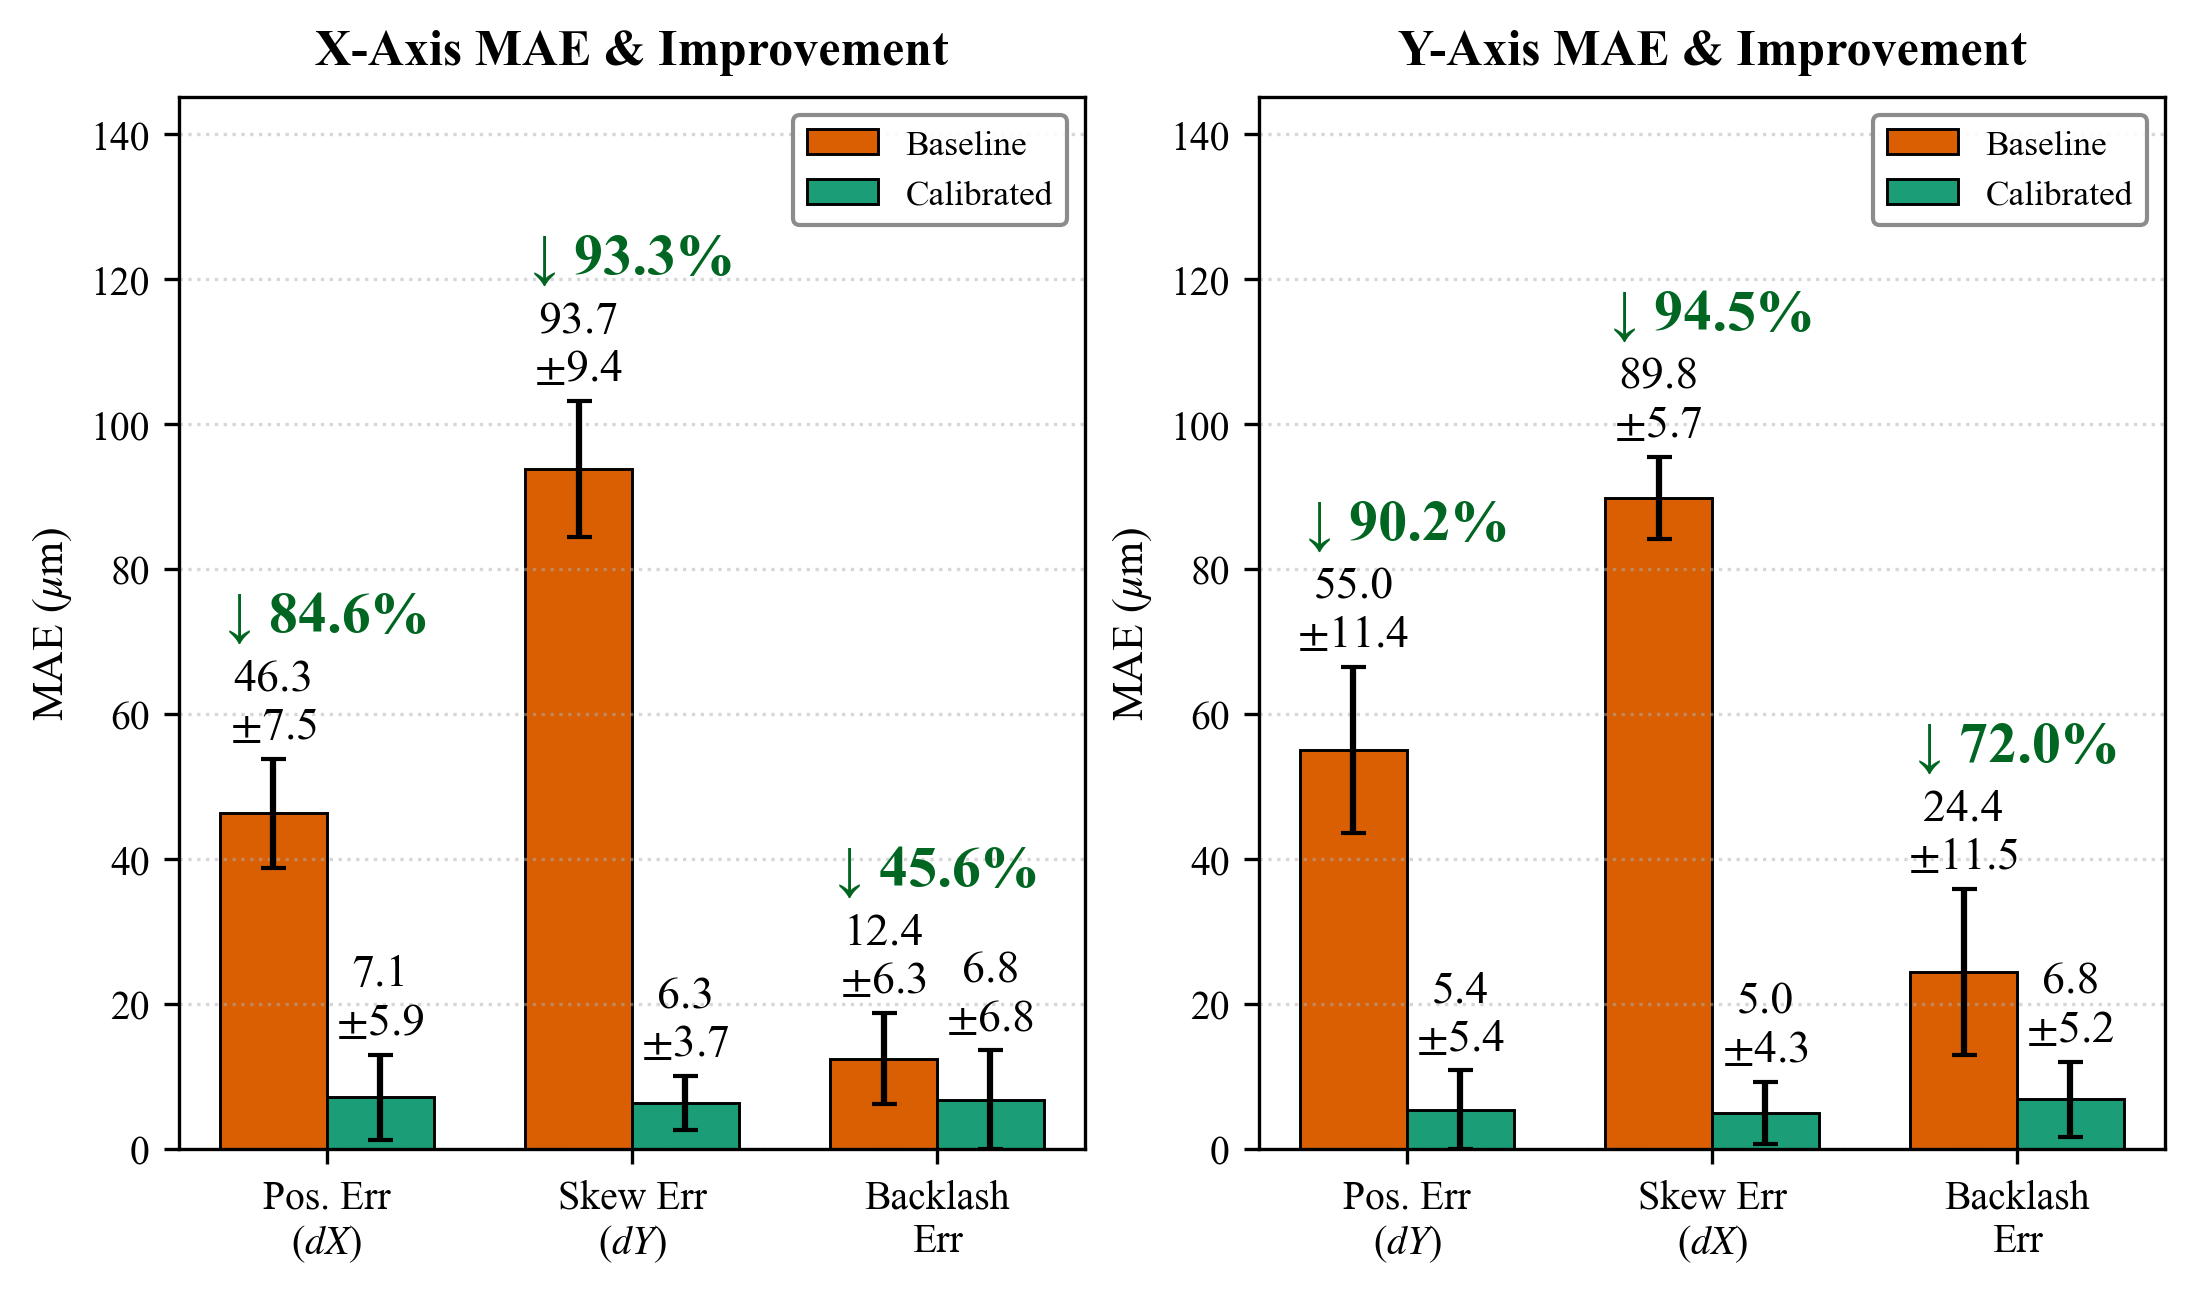
\includegraphics[width=1\linewidth]{images/mae_summary.png}
	\caption{Summary of Mean Absolute Errors (MAE) and percentage improvements across positioning, skew, and backlash metrics for X and Y axes.}
	\label{fig:maesum}
\end{figure}

\subsection{Simultaneous Trajectory Validation}
Dynamic tracking performance was evaluated by commanding the machine to trace a continuous elliptical trajectory, requiring synchronized, simultaneous motion across both axes. In the baseline state, the platform suffered from significant trajectory tracking deviations, resulting in an accumulated total Root Mean Square Error (RMSE) of $100.9 \pm 7.4~\mu$m.
Implementing the fine-tuned calibration parameters drastically corrected these trajectory deviations. The post-calibration X-axis tracking RMSE dropped to $34.42 \pm 1.70~\mu$m (a 55.25\% enhancement), while the Y-axis tracking RMSE was suppressed to $30.75 \pm 1.37~\mu$m (a 52.91\% enhancement). The total combined tracking error fell to $46.17 \pm 1.77~\mu$m, representing an overall trajectory accuracy improvement of 54.24\%. Visualization of the baseline performance and calibrated performance on one of the iterations while doing the trajectory movement shown in \figref{fig:vistrajectory}. The statistical result of the 10 iterations trajectory movement shown in \figref{fig:traj_rmse_iter} and \figref{fig:traj_summary_bars}.

\begin{figure}[!htbp]
	\centering
	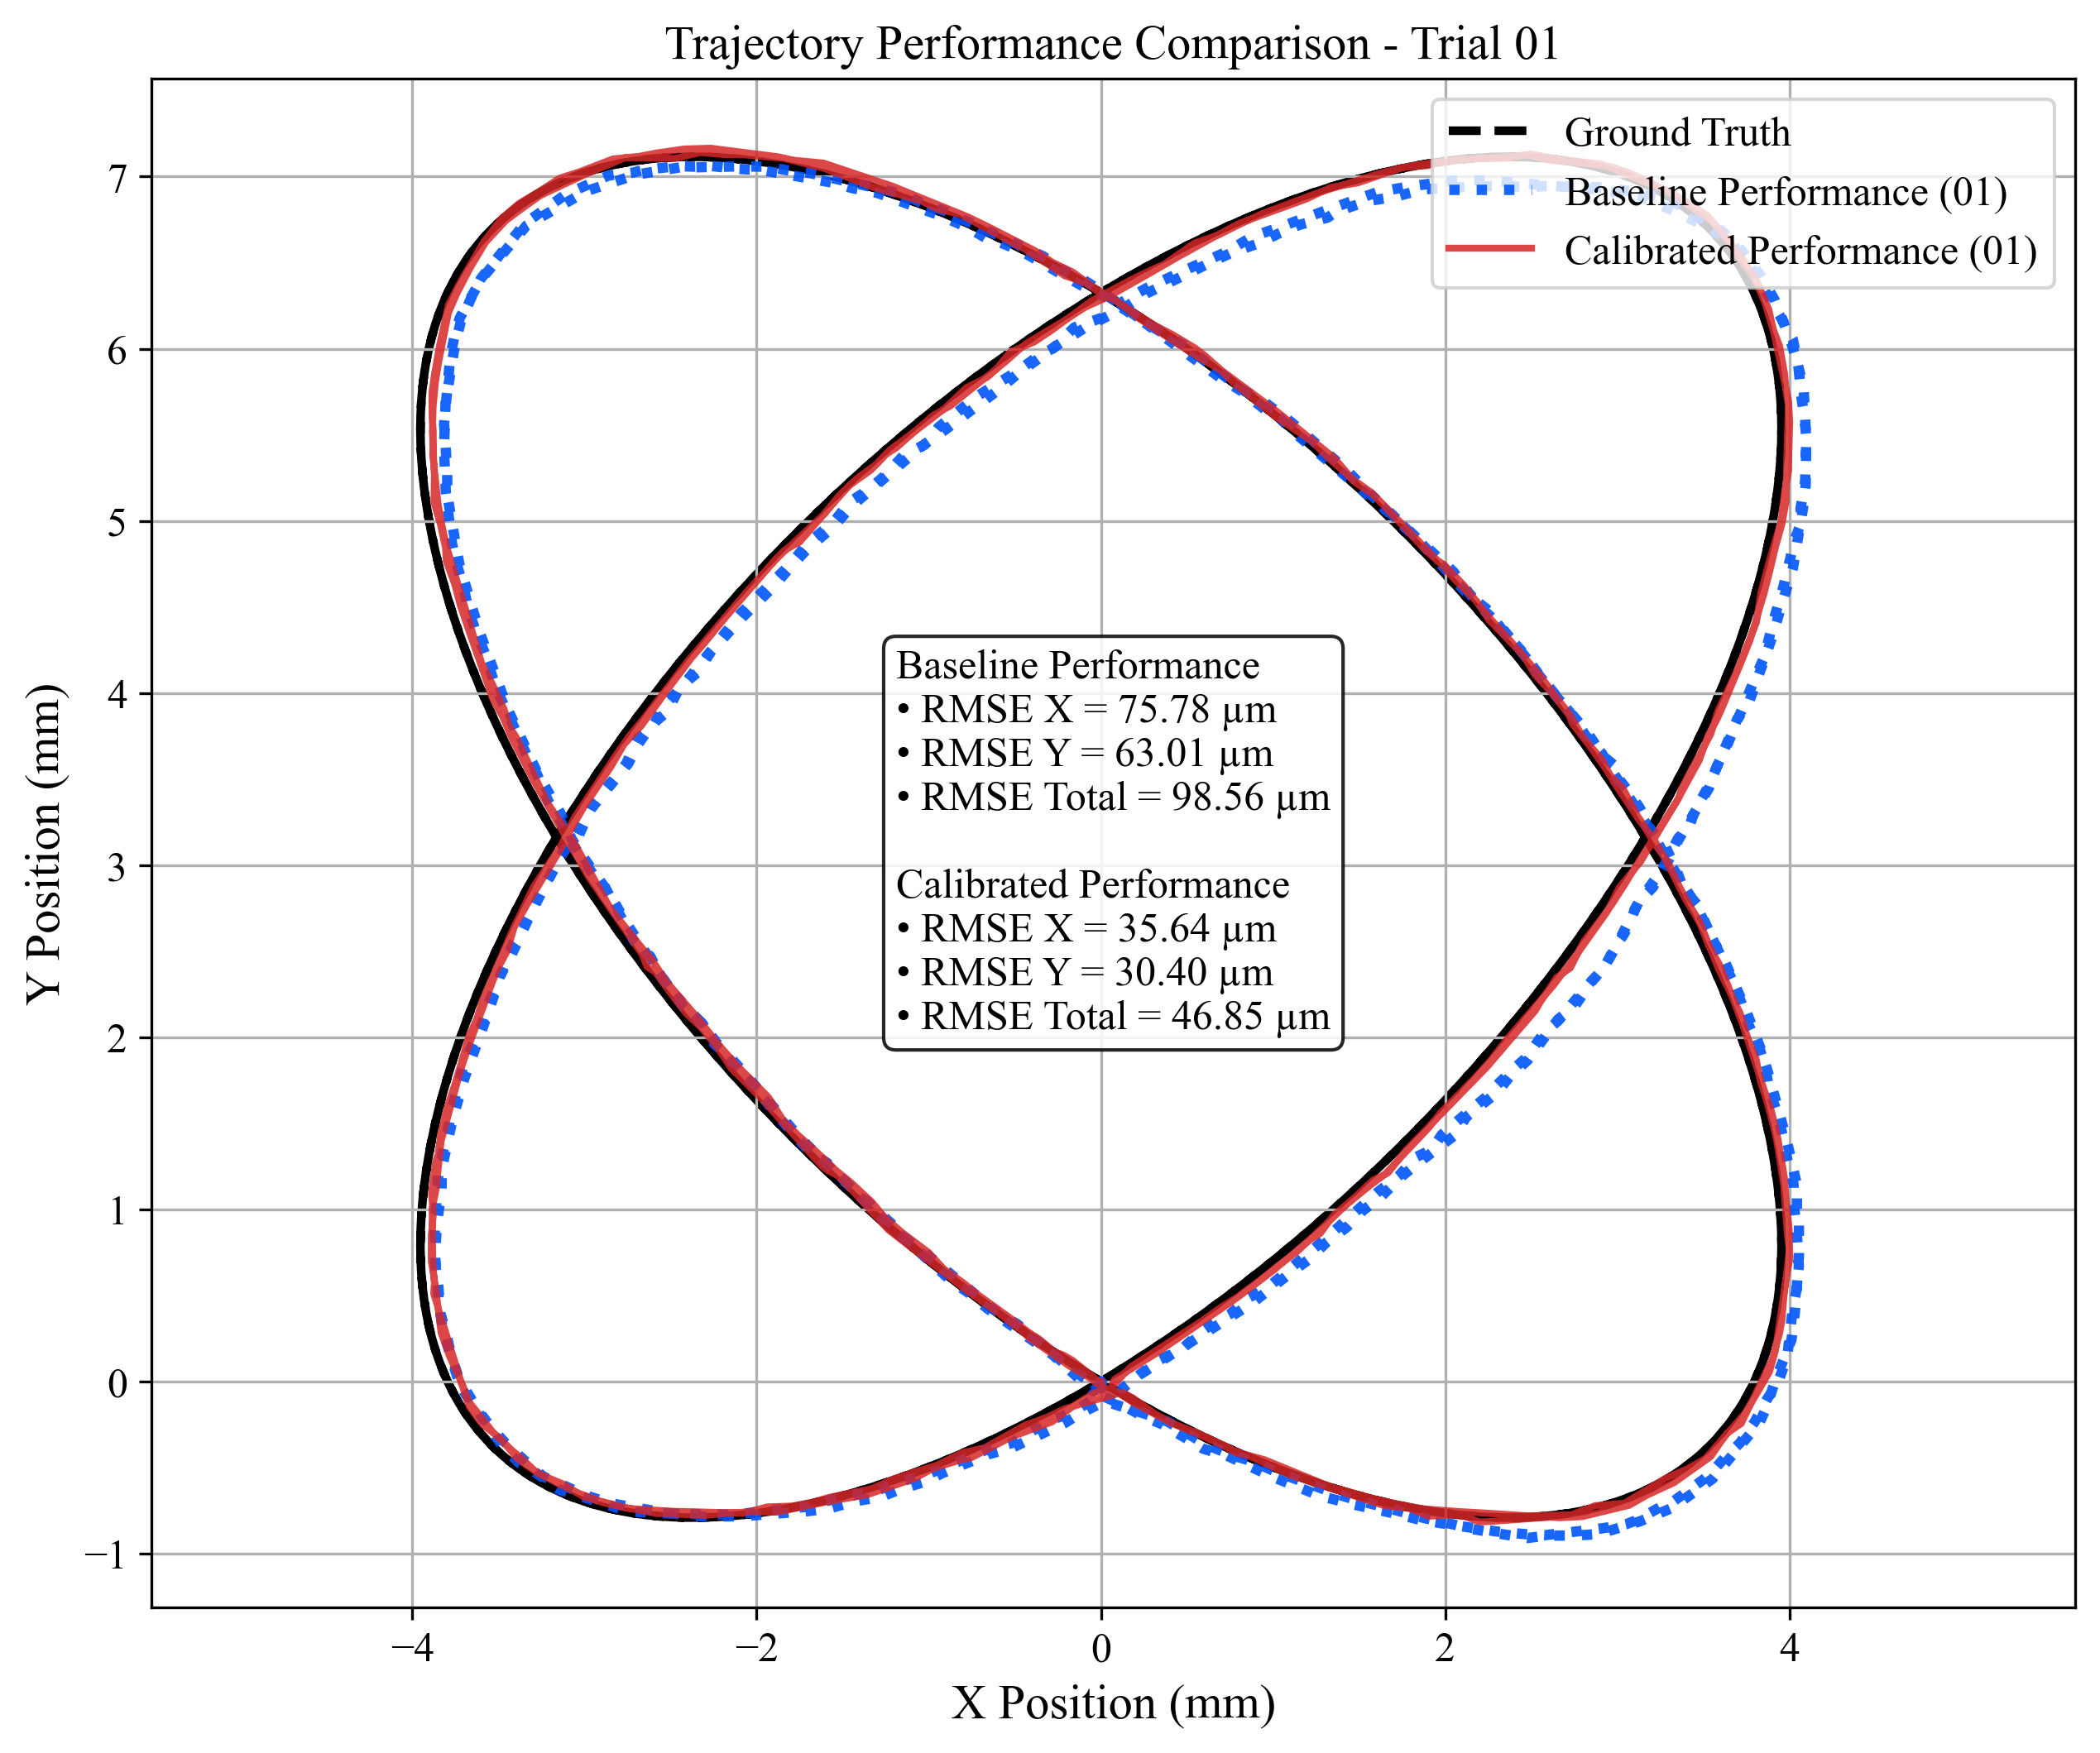
\includegraphics[width=1\linewidth]{images/perbandingan_full_01.png}
	\caption{Visualization of trajectory movement on baseline performance and calibrated performance.}
	\label{fig:vistrajectory}
\end{figure}

\begin{figure}[!htbp]
	\centering
	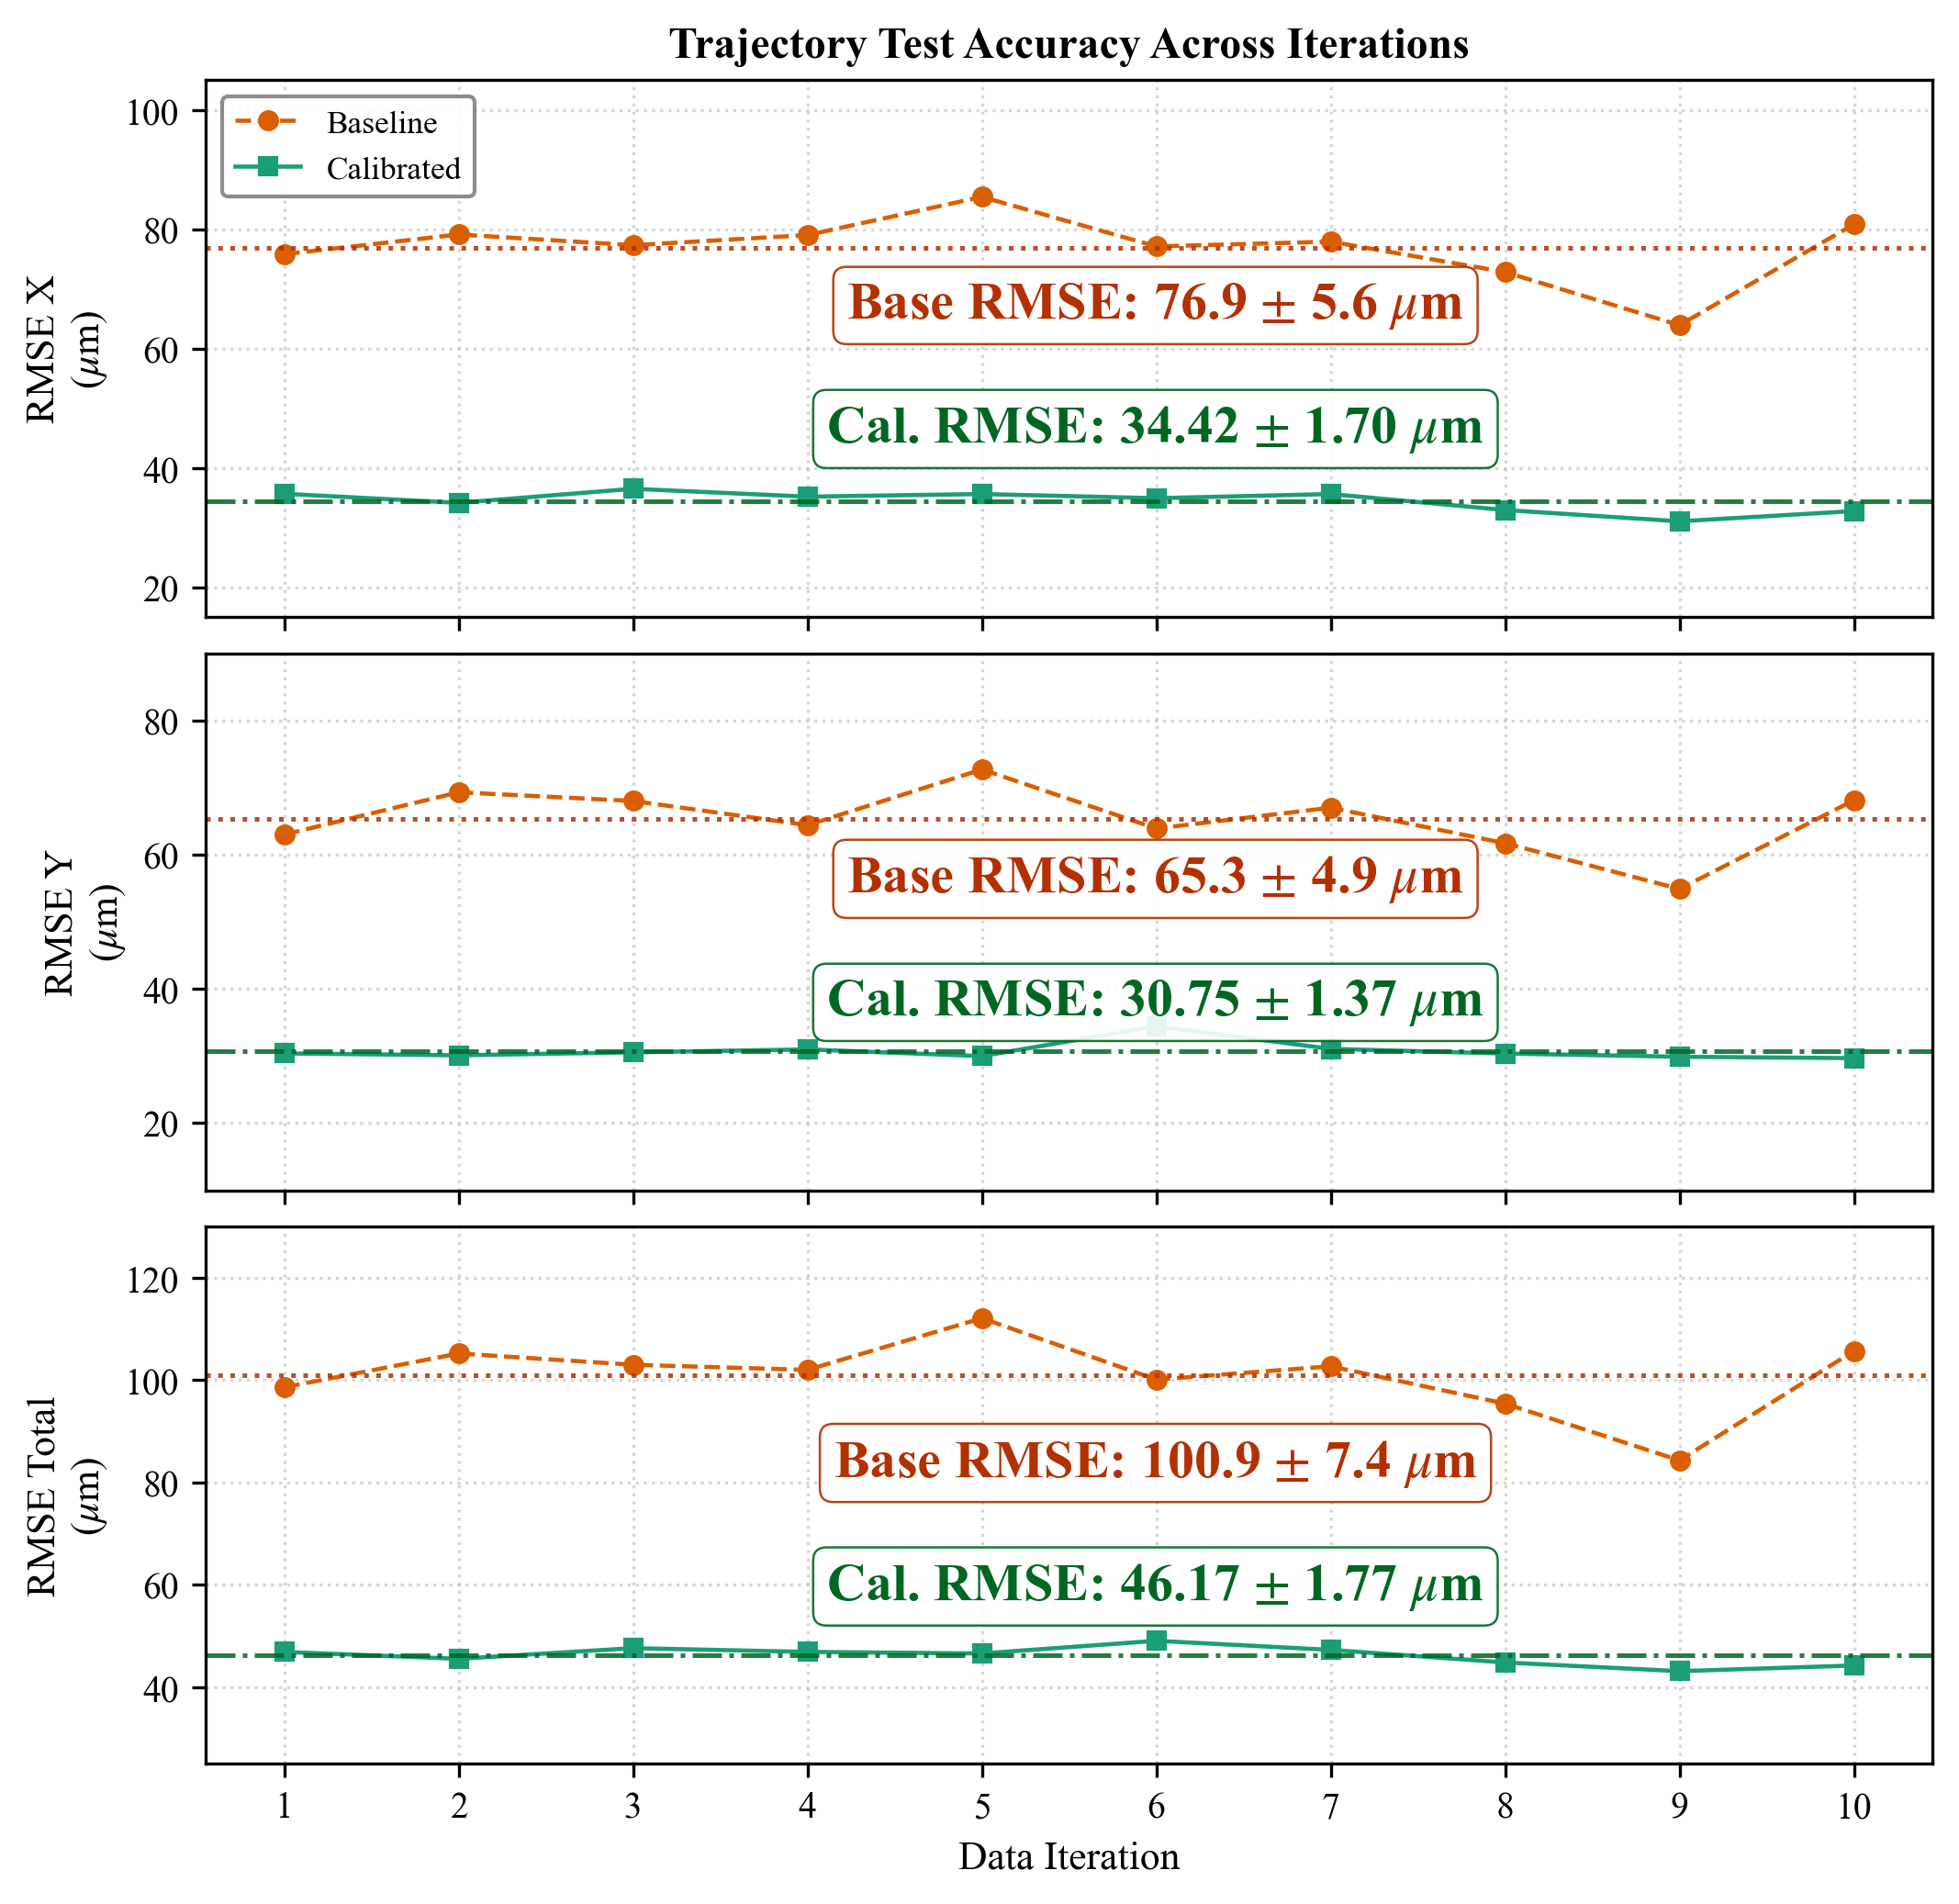
\includegraphics[width=1\linewidth]{images/trajectory_rmse_iterations_final.png}
	\caption{Tracking Root Mean Square Error (RMSE) across 10 iterations during continuous trajectory testing for X-axis, Y-axis, and total vector components.}
	\label{fig:traj_rmse_iter}
\end{figure}

\begin{figure}[!htbp]
	\centering
	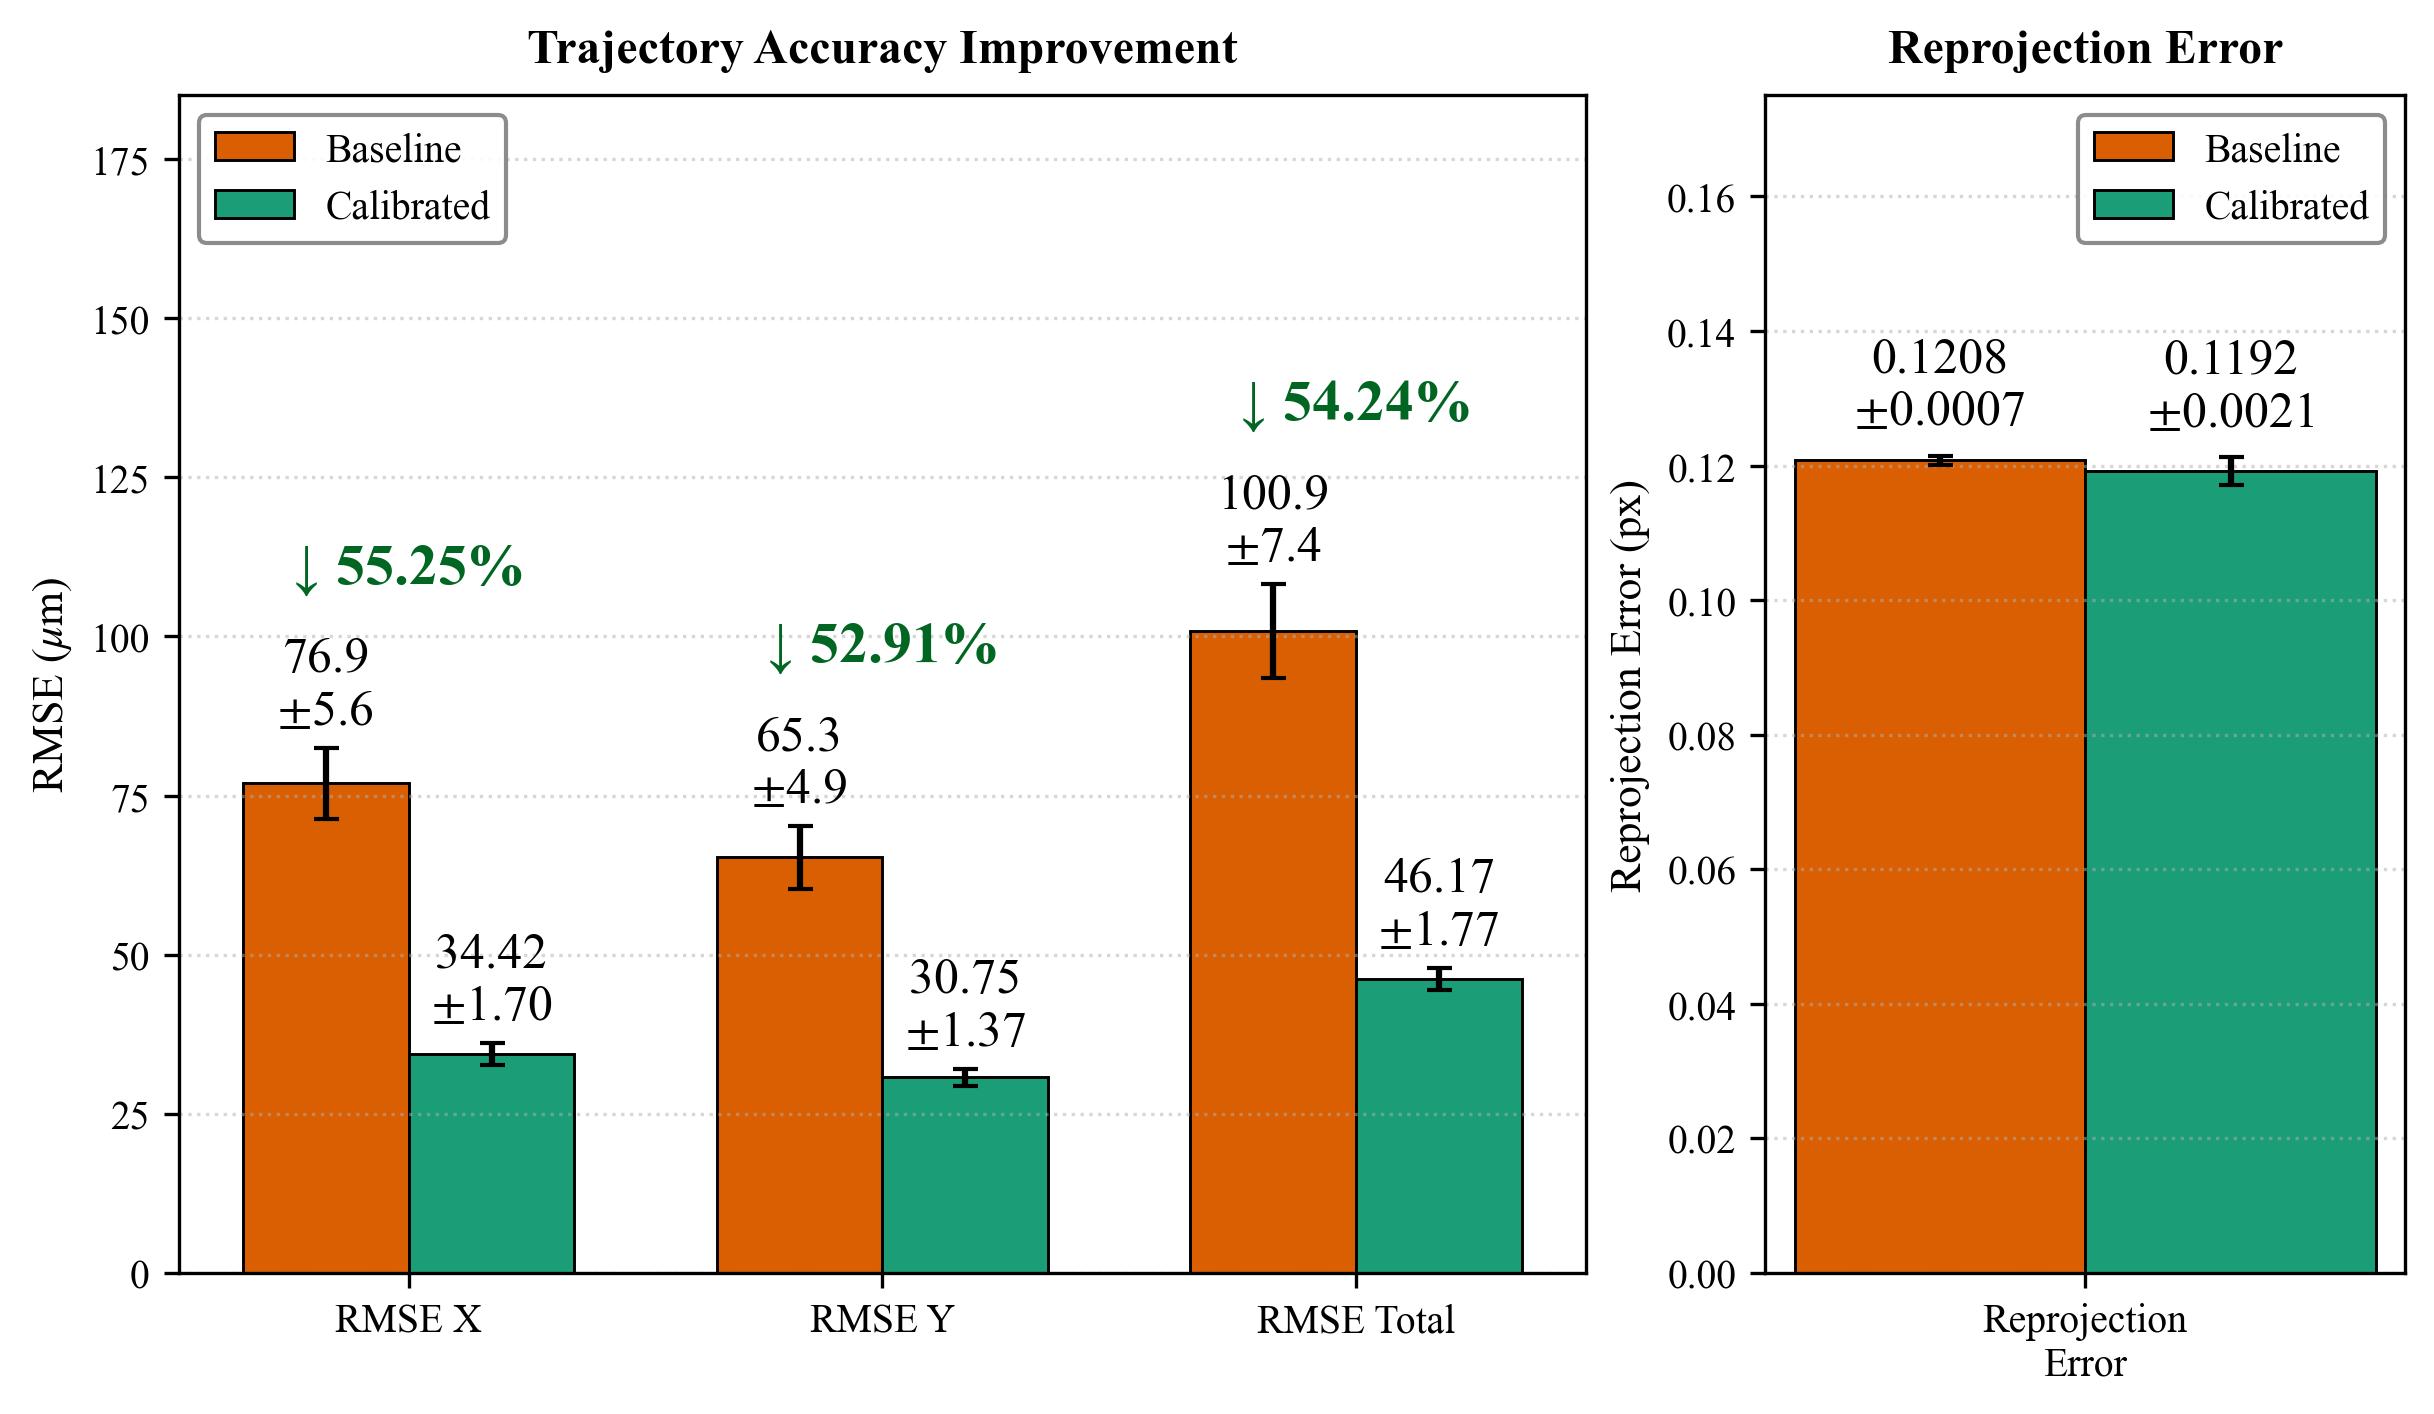
\includegraphics[width=1\linewidth]{images/trajectory_summary_bars_final.png}
	\caption{Statistical comparison of trajectory tracking accuracy improvements (RMSE X, Y, and Total) and reprojection error between baseline and calibrated system states.}
	\label{fig:traj_summary_bars}
\end{figure}

\subsection{Comparative Literature Analysis}
To evaluate commercial and scientific feasibility, the proposed virtual encoder was benchmarked against existing 3D printer calibration and kinematic measurement methodologies. Table~\ref{tab:literature_comparison} outlines the methodology performance, hardware requirements, and economic trade-offs across different approaches.

\providecommand{\newcolumntype}[2]{}
\newcolumntype{L}{>{\raggedright\arraybackslash}X}

\begin{table*}[ht]
	\centering
	\caption{Comparative Analysis of Calibration and Vision-Based Measurement Systems in Additive Manufacturing}
	\label{tab:literature_comparison}
	\scriptsize
	\setlength{\tabcolsep}{3pt}
	\renewcommand{\arraystretch}{1.2}
	
	\begin{tabularx}{\textwidth}{@{} L L L L L L @{}}
		\toprule
		\textbf{Category / Metric} & \textbf{Virtual Encoder (Proposed)} & \textbf{Owais et al. (2026) \cite{Owais2026}} & \textbf{Schouten et al. (2022) \cite{Schouten2022}} & \textbf{Chen \& Cai (2025) \cite{Chen2025}} & \textbf{Munteanu et al. (2021) \cite{Munteanu2021}} \\
		\midrule
		
		\textbf{Primary Domain} & 
		FDM Spatial Calibration \& Trajectory Tracking & 
		Spatial Vision Metrology \& Distortion & 
		Multi-Material Nozzle Offset Alignment & 
		Dual-Nozzle Spatial Auto-Calibration & 
		FDM Kinematic Error \& Trajectory Analysis \\
		
		\midrule
		\multicolumn{6}{@{}l}{\textbf{1. METHODOLOGY PERFORMANCE}} \\
		\midrule
		
		$\bullet$ \textbf{Measurement Error} & 
		$< 7~\mu\text{m} \mid 0.11\text{ px}$ & 
		$84~\mu\text{m} \mid 0.55\text{ px}$ & 
		$\approx 45~\mu\text{m}$ (Inductive vs. Optical) & 
		$< 100~\mu\text{m}$ ($0.1\text{ mm}$) & 
		Micron-level (Sensor resolution dependent) \\
		
		$\bullet$ \textbf{Positioning / Calibration} & 
		$8.92 \pm 5.42~\mu\text{m}$ & 
		$100 \pm 80~\mu\text{m}$ (Target region) & 
		$2~\mu\text{m}$ Inductive Repeatability & 
		$< 100~\mu\text{m}$ Nozzle Alignment & 
		$10 - 50~\mu\text{m}$ (Kinematic backlash / hysteresis) \\
		
		$\bullet$ \textbf{Dynamic Trajectory Tracking} & 
		Supported ($46.17 \pm 1.77~\mu\text{m}$ RMSE) & 
		N/A (Printed artifact: $30 \pm 20~\mu\text{m}$) & 
		N/A (Discrete Point Sensing) & 
		N/A (Static Nozzle Alignment) & 
		Supported (2D circular trajectory sampling) \\
		
		\midrule
		\multicolumn{6}{@{}l}{\textbf{2. HARDWARE REQUIREMENT}} \\
		\midrule
		
		$\bullet$ \textbf{Sensor / Camera Setup} & 
		1$\times$ Standard USB Monocular Camera & 
		Multi-Camera Rig (Stereo / Multi-view) & 
		Bed-Integrated Coil + A4 Scanner & 
		1$\times$ Internal Monocular Camera & 
		2$\times$ Non-Contact Optical Sensors \\
		
		$\bullet$ \textbf{Target / Physical Fixture} & 
		Planar Chessboard Target on Toolhead & 
		Volumetric Calibration Rig \& Artifacts & 
		Conductive Metallic Nozzle (Mandatory) & 
		Bed-Mounted Optical Prism \& LED Module & 
		External Calibration Reference Fixture \\
		
		$\bullet$ \textbf{Computing Infrastructure} & 
		External Host PC \& Standard MCU (Marlin) & 
		Vision Metrology Workstation & 
		Embedded MCU + PC Image Processing & 
		Integrated Compute Module / Host PC & 
		External DAQ System \& Computer Processing \\ 
		
		\midrule
		\multicolumn{6}{@{}l}{\textbf{3. ECONOMIC TRADE-OFFS}} \\
		\midrule
		
		$\bullet$ \textbf{Module Hardware Cost} & 
		Low ($\sim\$10 - \$25$) & 
		Medium -- High (Multi-camera rig) & 
		Very Low (PCB coil) / Scanner extra & 
		Low -- Medium (Standard camera) & 
		Medium -- High (Specialized optical sensors) \\
		
		$\bullet$ \textbf{MCU Computational Load} & 
		None (Offloaded to Host PC) & 
		Heavy (Offline multi-view processing) & 
		Very Light (Real-time inductance) & 
		Medium (Hough/Color Segmentation) & 
		None (External DAQ system processing) \\
		
		$\bullet$ \textbf{Implementation Complexity} & 
		Low -- Medium (Monocular \& planar target) & 
		High (Multi-camera stereo alignment) & 
		Medium (Print bed modification) & 
		Low (Bed-mounted prism \& camera setup) & 
		Medium (Rigid sensor mounting \& alignment) \\
		
		$\bullet$ \textbf{Automation \& Efficiency} & 
		Automated Data Acquisition and Offline Frame Analysis & 
		Offline Metrology Mapping & 
		Automated (Inductive) / Manual (Paper) & 
		Automated (Pre-print routine) & 
		Offline Trajectory Signal Analysis \\
		
		\bottomrule
	\end{tabularx}
\end{table*}